\documentclass[final]{beamer}
\usetheme{IST}
\usepackage[orientation=portrait,size=a0,scale=1.4,debug]{beamerposter}  % poster size
\usepackage[absolute,overlay]{textpos}
\usepackage[utf8]{inputenc}
\usepackage{graphicx,caption,subcaption,float,lipsum}
\captionsetup[subfigure]{labelformat=empty}
\graphicspath{ {./images/} }

\setlength{\TPHorizModule}{1cm}
\setlength{\TPVertModule}{1cm}

\title{eNM-Ontoviewer: Interactive visualisation of SPARQL queries for eNanoMapper ontologies and data}
\author{D. Gebele, M. Rautenberg, C. Helma}
\institute{\emph{in silico} toxicology gmbh, Basel, Switzerland}
\footer{Contact: \texttt{support@in-silico.ch}. Information: \texttt{www.in-silico.ch}}

\begin{document}

  \begin{frame}{}

    \begin{textblock}{81.5}(1,12)
      \justifying
      \input{./markdown_blocks/ontoviewer_summary}
    \end{textblock}
    
    \begin{textblock}{30}(1,20)
      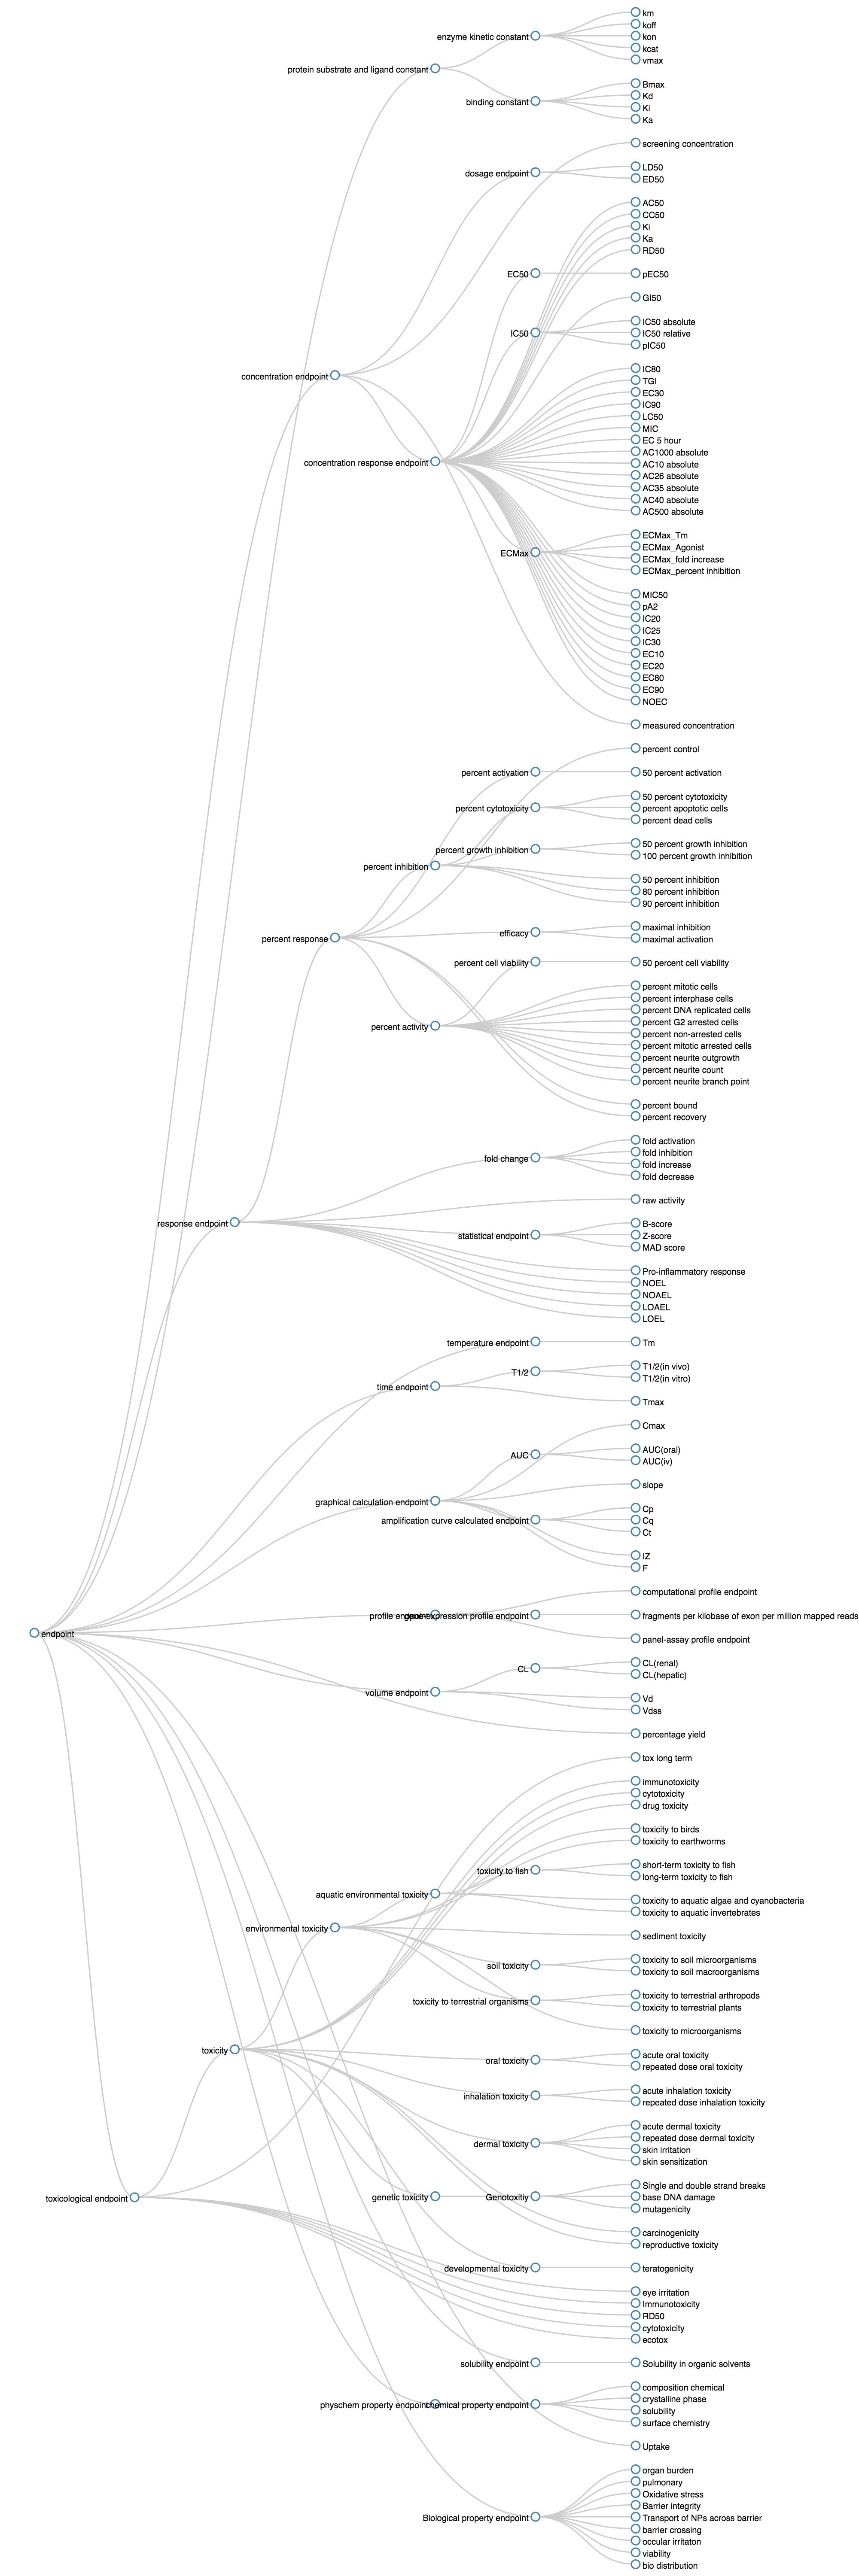
\includegraphics[scale=0.35,trim={20cm 0 0 0},clip]{onto-viewer-dendogram-1.png}
    \end{textblock}
    \begin{textblock}{40}(3,96)
      \small Figure 1: Dendogram
    \end{textblock}
    
    \begin{textblock}{63}(20,18)
      \justifying
      \begin{block}{Use case 1: Investigate the eNanoMapper ontology}
        Assuming that we are interested in \emph{toxicological endpoints} we execute the template SPARQL query to receive results either as a static \emph{Dendogram} graph \emph{(Figure 1)} or as an interactive \emph{Sunburst} graph \emph{(Figure 2)}. To get all information about a subject we can use the SPARQL interface \emph{(Figure 4)} and write another query. We are always able to refine our query or investigate directly any kind of URIs from the result \emph{(Figure 5)}.
        \begin{figure}
          \hspace{-0.1\textwidth}
          \begin{subfigure}[c]{0.35\textwidth}
            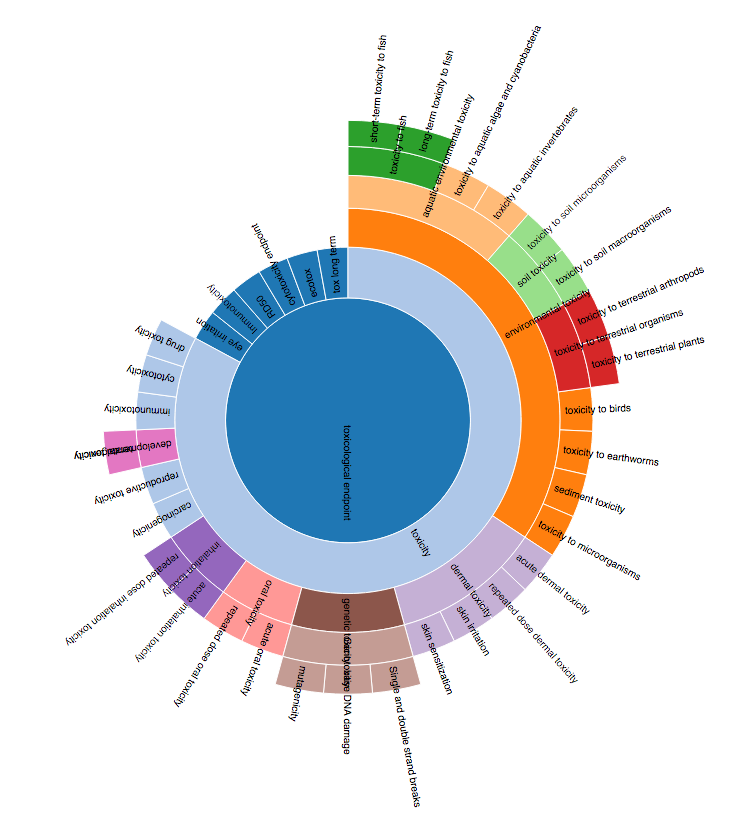
\includegraphics[scale=0.75,keepaspectratio]{onto-use-case-1a.png}
            \caption{Figure 2: Sunburst. Result for \emph{toxicological endpoint} search.}
          \end{subfigure}
          \hspace{0.15\textwidth}
          \begin{subfigure}[c]{0.35\textwidth}
            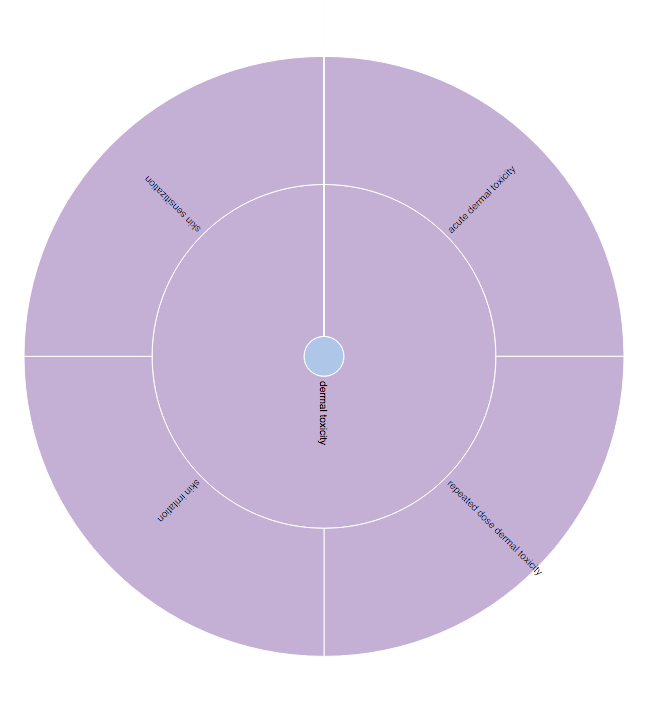
\includegraphics[scale=0.65,keepaspectratio]{onto-use-case-1b.png}
            \caption{Figure 3: Sunburst. Interactive zoom on \emph{dermal toxicity} endpoint.}
          \end{subfigure}
        \end{figure}
        \vspace{0.02\textwidth}
        \begin{figure}
          \hspace{-0.1\textwidth}
          \begin{subfigure}[c]{0.35\textwidth}
            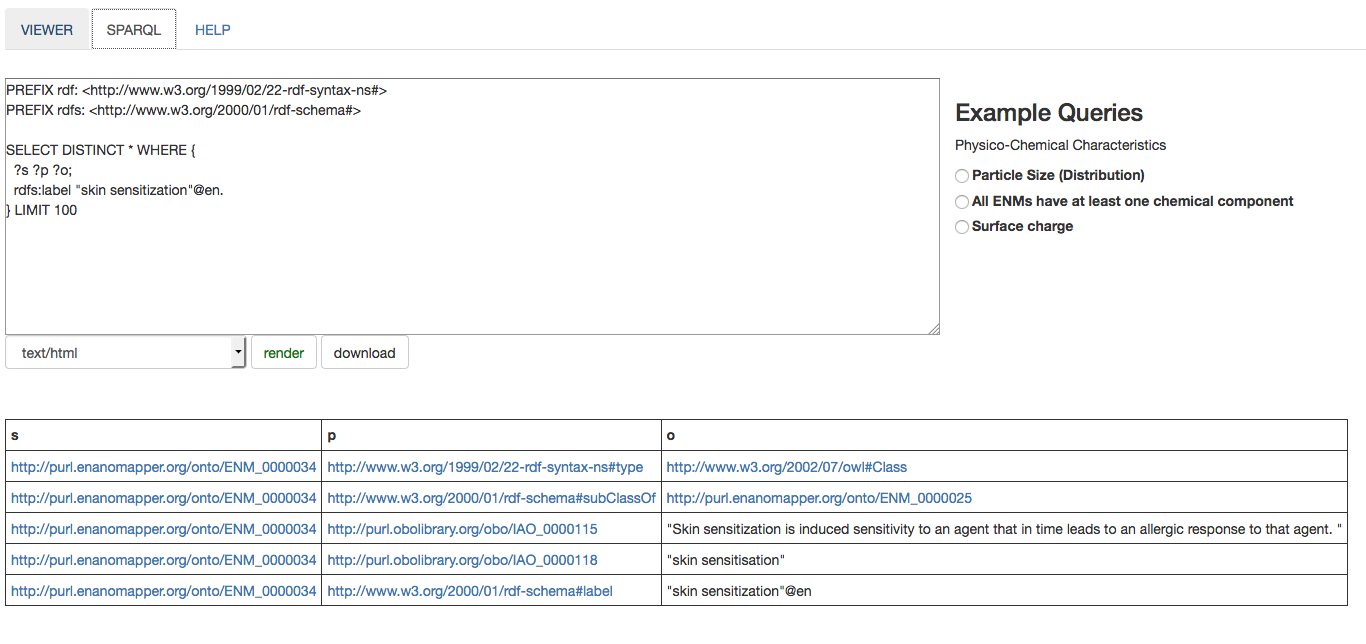
\includegraphics[scale=0.5,keepaspectratio]{onto-use-case-1c.png}
            \caption{Figure 4: SPARQL interface. Select \emph{skin sensitization} subclass endpoint from \emph{Figure 3} for a detail query.}
          \end{subfigure}
          \hspace{0.12\textwidth}
          \begin{subfigure}[c]{0.35\textwidth}
            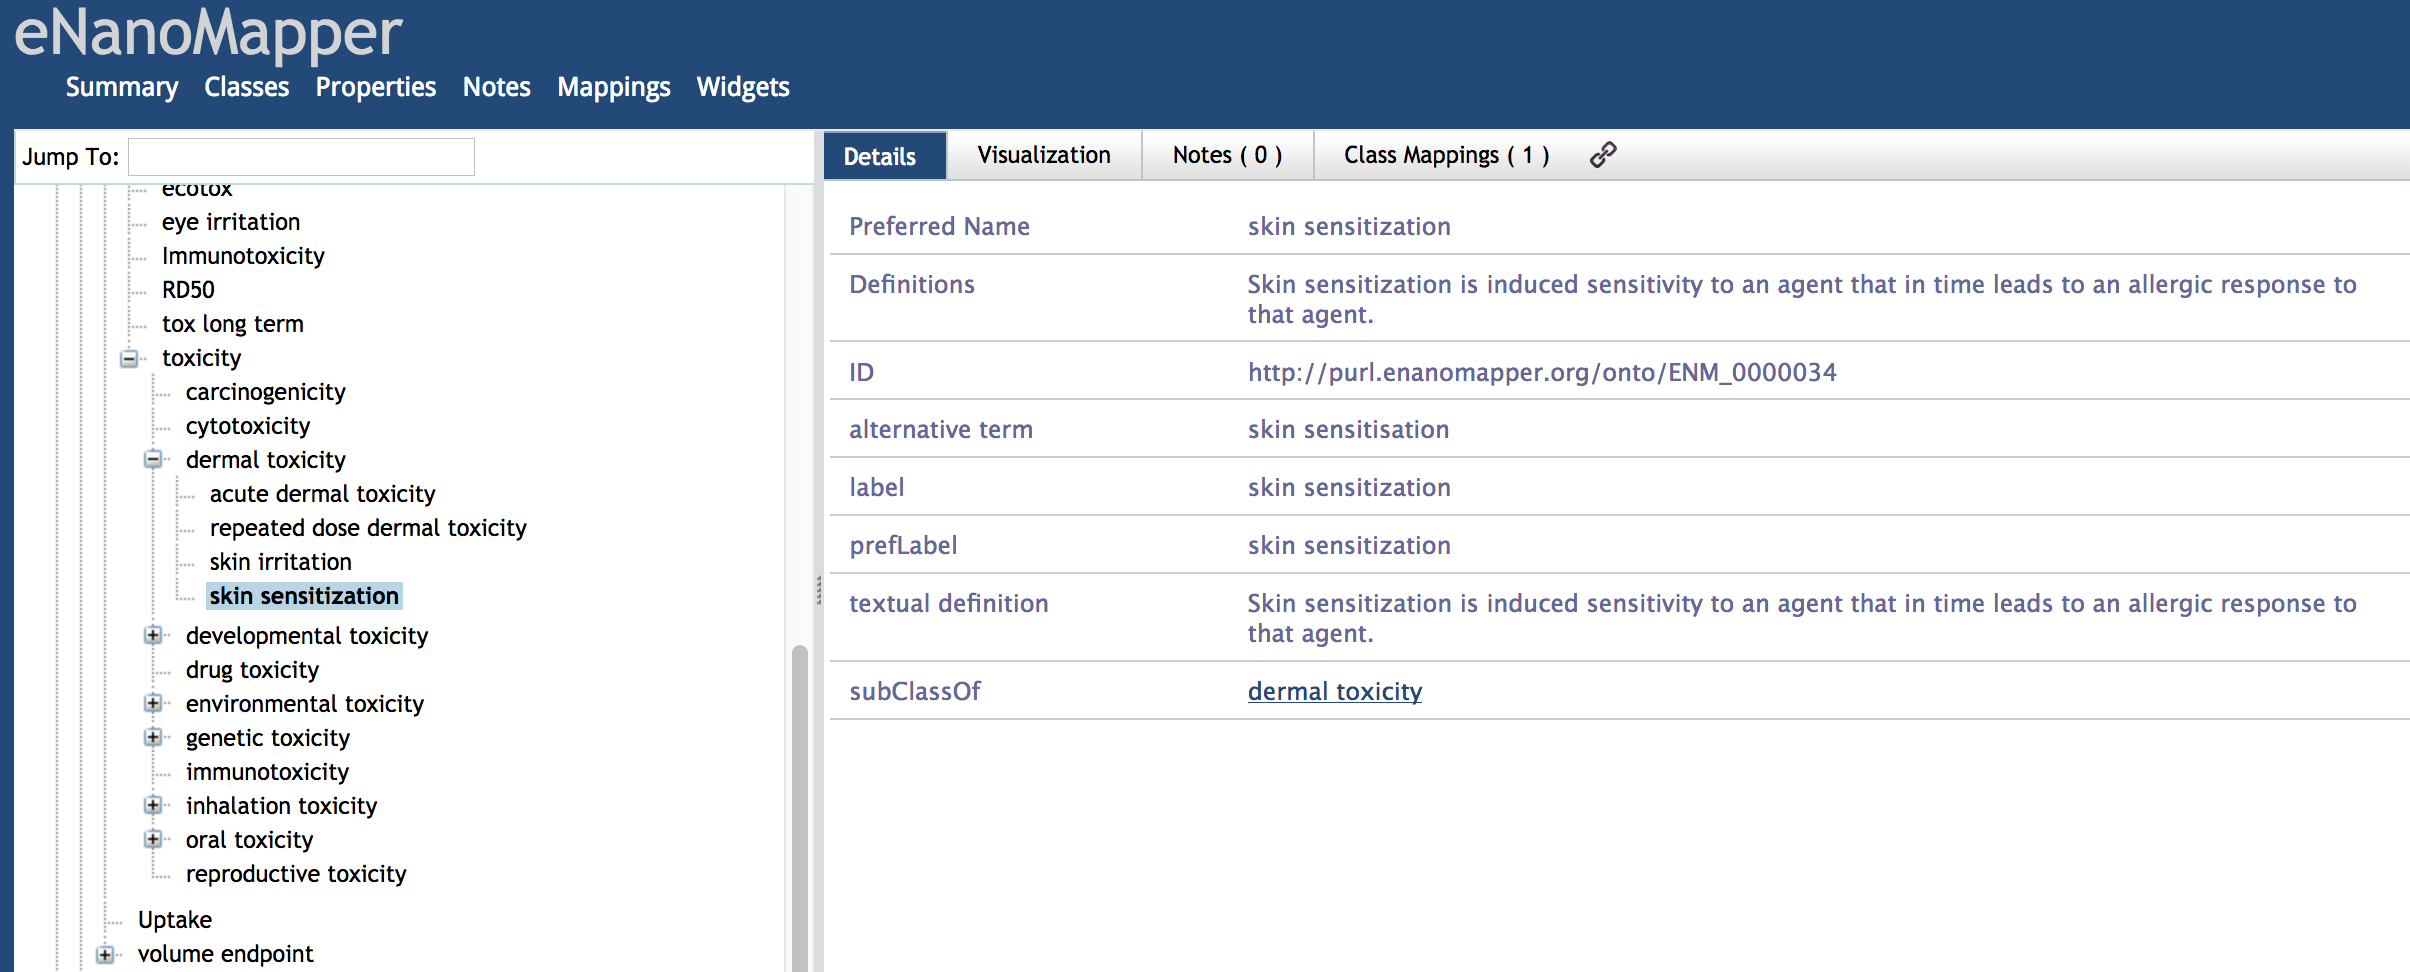
\includegraphics[scale=0.6,keepaspectratio]{onto-use-case-1d.png}
            \caption{Figure 5: Following a link from the query result in \emph{Figure 4} we reach the eNanoMapper ontology on BioPortal.}
          \end{subfigure}
        \end{figure}
      \end{block}
    \end{textblock}

        
    \begin{textblock}{63}(20,70)
      \justifying
      \begin{block}{Use case 2: Investigate eNanoMapper data}
        Assuming that we want to investigate eNanoMapper nano material data we can simply choose one of the given SPARQL examples \emph{(Figure 6)} as a starting point. In this case we are interested in \emph{surface charge} and search for the zeta potential and its values. We receive a table with values and resource identifiers which point us directly to the resource page of the eNanoMapper database service \emph{(Figure 7)}.
        \begin{figure}
          \vspace{0.01\textwidth}
          \hspace{-0.15\textwidth}
          \begin{subfigure}[c]{0.35\textwidth}
            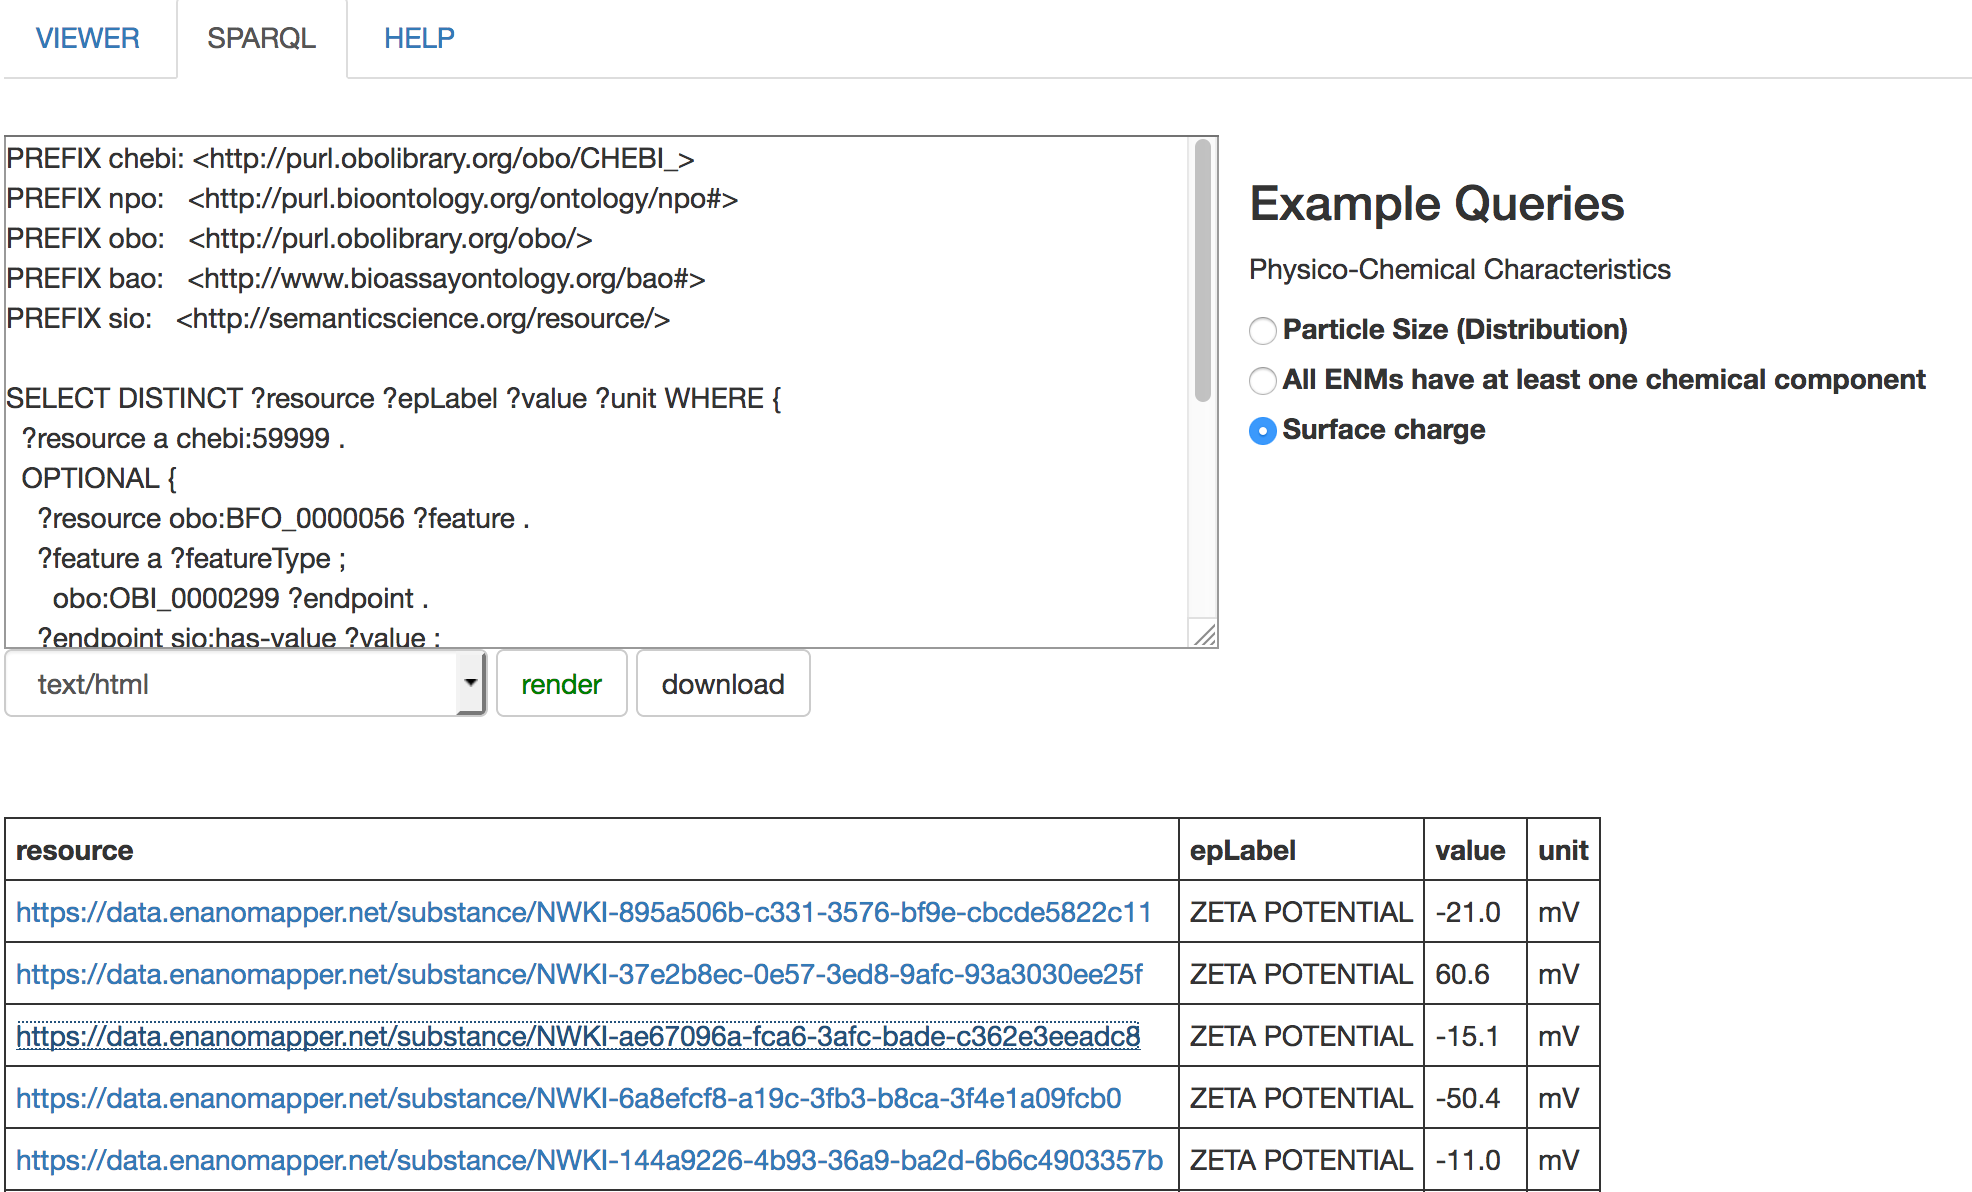
\includegraphics[scale=0.75,keepaspectratio]{onto-use-case-2a.png}
            \caption{Figure 6: SPARQL interface. Select one of the \emph{physio-chemical characteristics} examples.}
          \end{subfigure}
          \hspace{0.12\textwidth}
          \begin{subfigure}[c]{0.35\textwidth}
            \vspace{0.1\textwidth}
            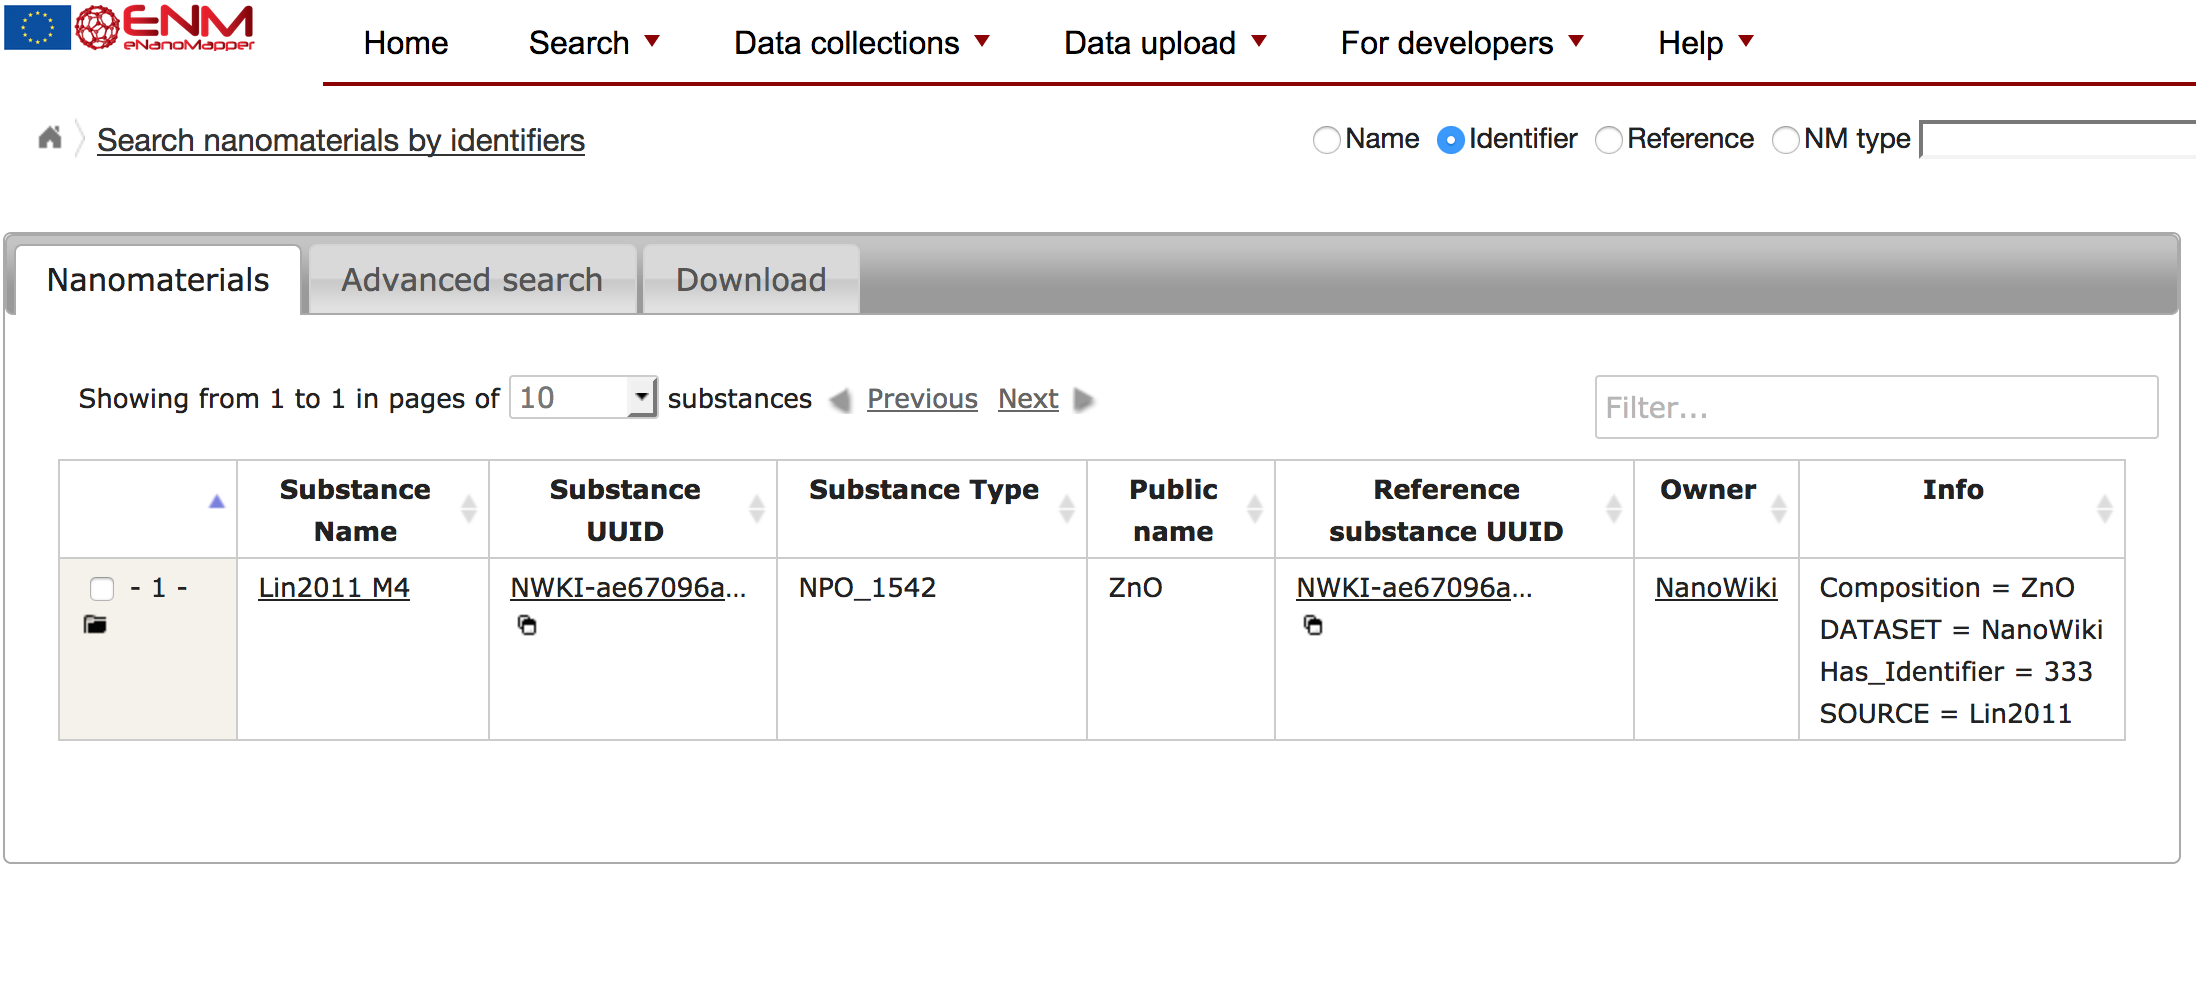
\includegraphics[scale=0.75,keepaspectratio]{onto-use-case-2b.png}
            \caption{Figure 7: Following a link from the query result in \emph{Figure 6} we reach the eNanoMapper database service.}
          \end{subfigure}
        \end{figure}
      \end{block}
    \end{textblock}
    
    \begin{textblock}{39.5}(1,100)
      \begin{exampleblock}{Links}
        \input{./markdown_blocks/ontoviewer_links}
      \end{exampleblock}
    \end{textblock}

    \begin{textblock}{40.5}(42.5,100)
      \begin{block}{References}
        \small\bibliography{references}
      \end{block}
    \end{textblock}

  \end{frame}

\end{document}
